\problem{Image Restoration}
(a) The spectrum of the origin image is generated through FFT.\\
To shift the zero frequency to the center of the spectrum, we times $(-1)^{u+v}$ for each pixel $(u,v)$ on the origin image before applying FFT.

To have a better effect of visualization on the frequency domain, the image is shown by applying the log transformation on the magnitude of the Fourier transform of the image.\\
i.e. $I_{\text{log}}=\log(1+|I|)$, where $I$ is the spectrum generated by Fourier transform of the image.\\
The spectrum of the origin image after fftshift is shown in Figure \ref{fig:p4a}.\\
\begin{figure}[htbp]
    \centering
	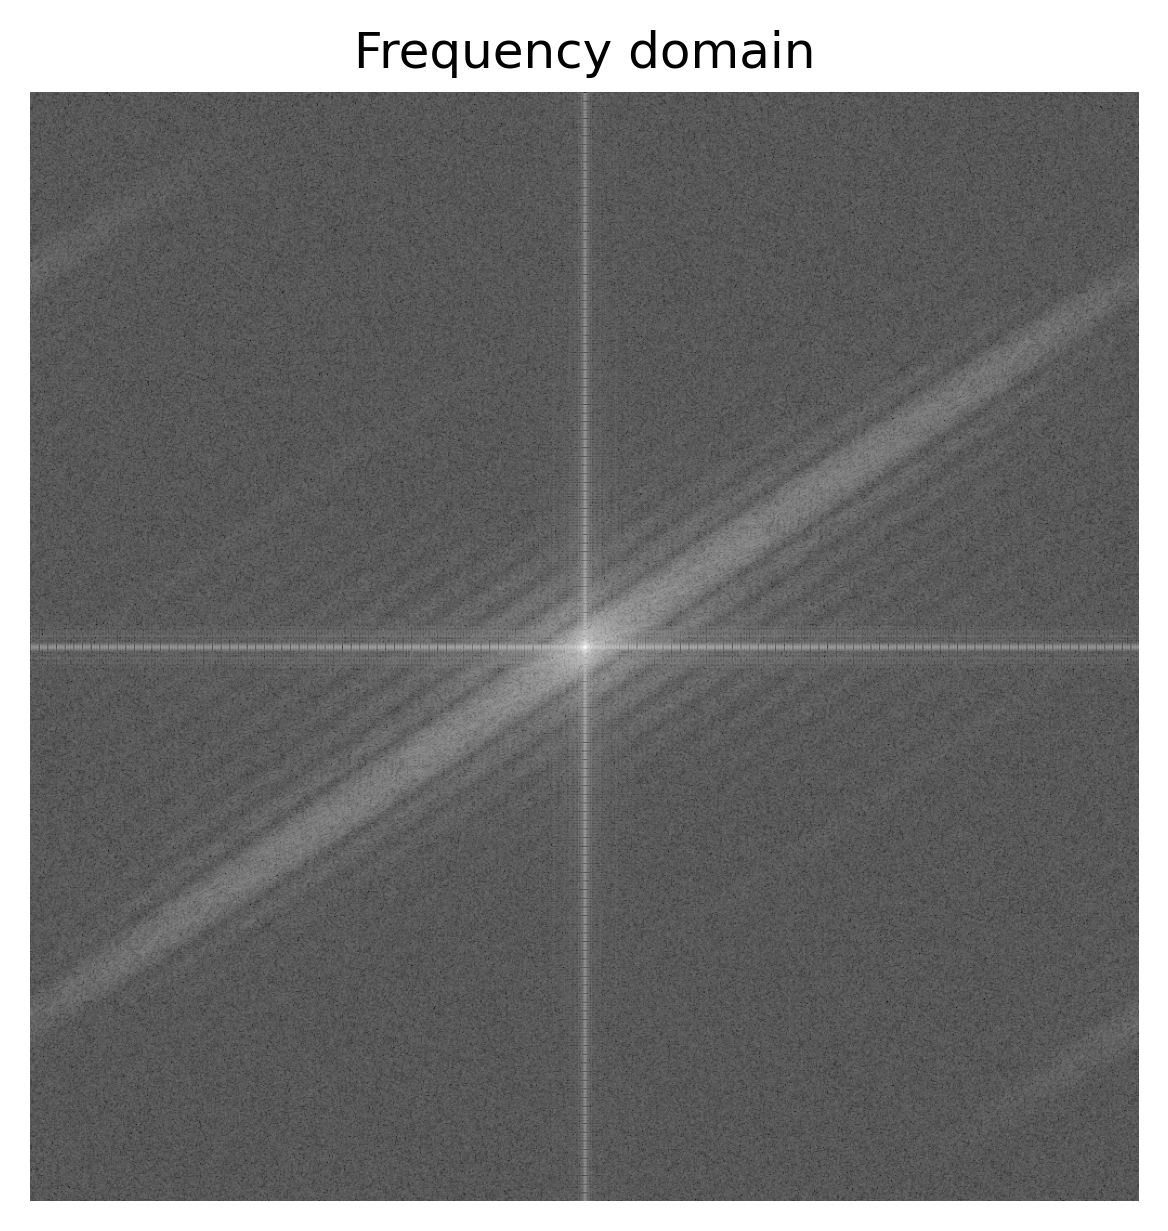
\includegraphics[width=0.5\textwidth]{../images/p4/p4a.png}
    \caption{FFT shifted spectrum}
    \label{fig:p4a}
\end{figure}

(b) Then we can apply transformation on the spectrum to get $theta$ and $d$ for the strip.\\
The Radon transform is:
$$g(\rho, \theta)=\sum_{x=0}^{M-1}\sum_{y=0}^{N-1}f(x,y)\delta(x\cos\theta+y\sin\theta-\rho)$$
where $\delta$ is the Dirac delta function.\\
$\rho_{\text{max}}=\lceil\dfrac{\sqrt{2}}{2}N\rceil=453$, so the vertical index is in range $[-\rho_{\text{max}},\rho_{\text{max}}]$.

The image by applying Radon transform on the origin image is shown in Figure \ref{fig:p4b_radon}.\\
We can get the horizontal coordinate with the highest intensity in the Radon transformed image, which is $\theta=124^{\circ}$.
\begin{figure}[htbp]
    \centering
	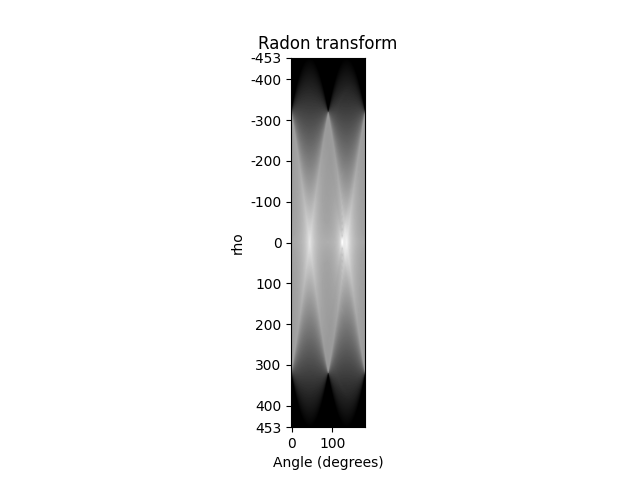
\includegraphics[width=0.8\textwidth]{../images/p4/p4b_radon.png}
    \caption{Radon Transformed image}
    \label{fig:p4b_radon}
\end{figure}

The we rotate the spectrum by $180^{\circ}-\theta=56^{\circ}$, and do vertical projection to find the distance between two similar dark strips.\\
The rotated spectrum and the intensity of the vertical projection are shown in Figure \ref{fig:p4b}.\\ 

\begin{figure}[htbp]
    \centering
	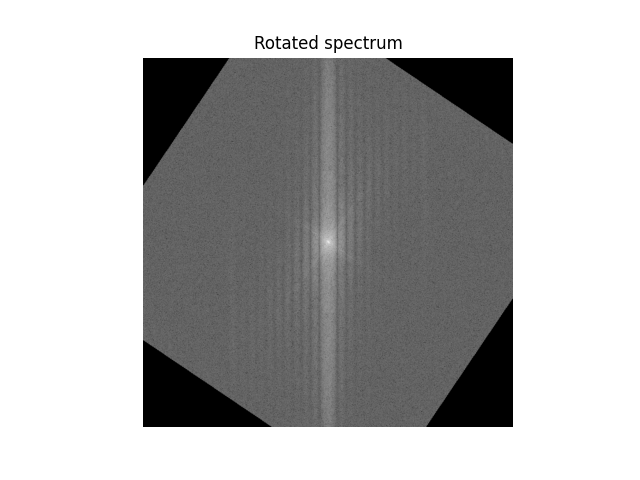
\includegraphics[width=0.48\textwidth]{../images/p4/p4b_rotated_image.png}
	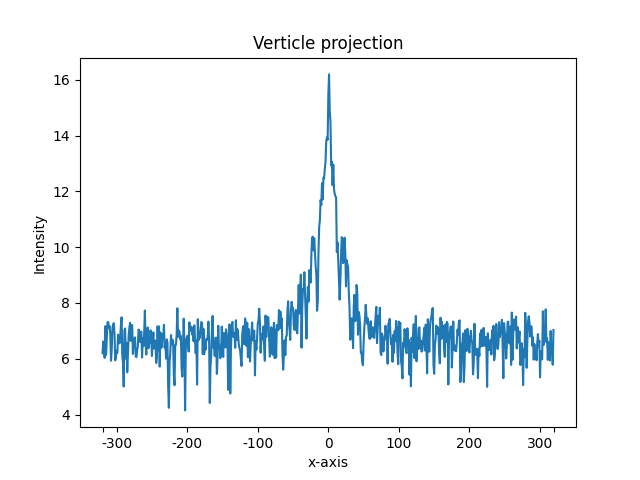
\includegraphics[width=0.48\textwidth]{../images/p4/p4b_intensity.png}
    \caption{Radon Transformed image}
    \label{fig:p4b}
\end{figure}
From Figure \ref{fig:p4b}, we can see that the two similar dark strips are $d=16$ pixels apart.\\
So we have $N=640,L=\dfrac{N}{d}=40$.

So above all, the parameters of the motion blur are $\theta=124^{\circ},L=40$.\\

(c)
We construct the frequency domain Wiener filter using the formula:
$$W = \dfrac{H^*}{|H|^2+K}$$
where $H$ is the Fourier transform of the point spread function, which was generated by the motion blur model with parameters $\theta=124^{\circ},L=40$. And the help of `psf2otf'.\\ 
We here take $K=0.004$, and we do not apply `fftshift' during the filtering.
Then the restored image by applying Wiener filter is shown in Figure \ref{fig:p4c}.\\
\begin{figure}[htbp]
    \centering
	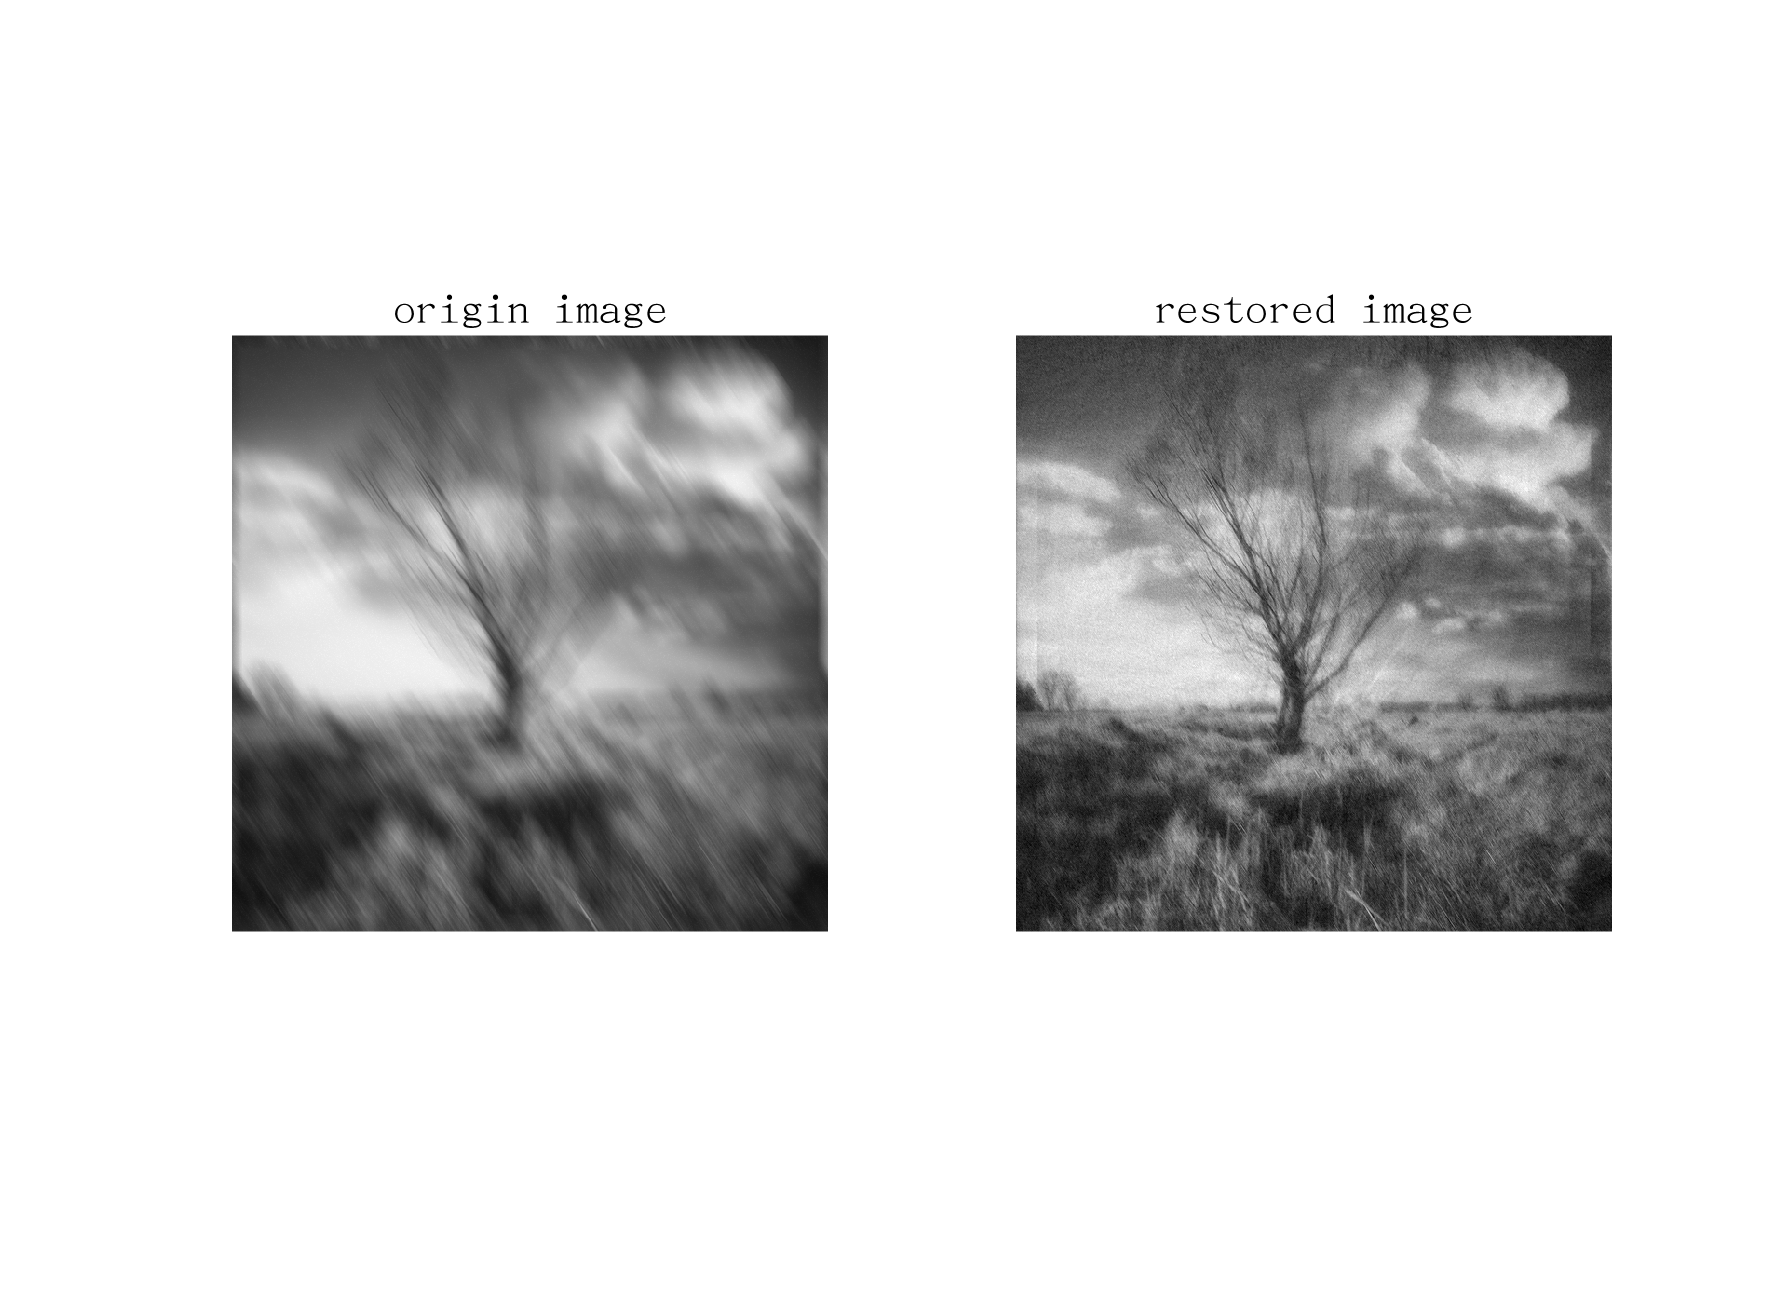
\includegraphics[width=\textwidth]{../images/p4/p4c.png}
    \caption{Restored image}
    \label{fig:p4c}
\end{figure}